\documentclass[conference]{IEEEtran}
\IEEEoverridecommandlockouts
% The preceding line is only needed to identify funding in the first footnote. If that is unneeded, please comment it out.
\usepackage{cite}
\usepackage{url}
\usepackage[english]{babel}
\usepackage{amsmath,amssymb,amsfonts}
\usepackage{algorithmic}
\usepackage{graphicx}
\usepackage{subcaption}
\graphicspath{ {./images/} }
\usepackage{textcomp}
\usepackage{xcolor}
\usepackage{tabularx}
\def\BibTeX{{\rm B\kern-.05em{\sc i\kern-.025em b}\kern-.08em
    T\kern-.1667em\lower.7ex\hbox{E}\kern-.125emX}}
\begin{document}

\title{Recurrent Neural Network Language Model Implementation\\
% {\footnotesize \textsuperscript{*}Note: Sub-titles are not captured in Xplore and
% should not be used}
% \thanks{Identify applicable funding agency here. If none, delete this.}
}

\author{\IEEEauthorblockN{Davide Lusuardi}
\IEEEauthorblockA{
    \textit{Department of Information Engineering and Computer Science} \\
    \textit{University of Trento}\\
    % University of Trento\\
Trento, Italy \\
davide.lusuardi@studenti.unitn.it}
}

\maketitle

\begin{abstract}

Language models are central to many Natural Language Processing (NLP) tasks as they can 
provide word representation and probability indication of word sequences. Some of these 
tasks include Machine Translation and Speech Recognition. Recurrent Neural Network 
Language Models (RNNLMs) improve the performance of traditional Language Models. In this 
work, we show how to implement a Recurrent Neural Network Language Model using PyTorch 
along with the implementation of simple LSTM and GRU cells. This report also shows the 
performance obtained on the Penn Tree-bank dataset using the perplexity metric (PPL).

\end{abstract}

% \begin{IEEEkeywords}
% component, formatting, style, styling, insert
% \end{IEEEkeywords}

\section{Introduction}
Language modeling task consists in predicting the probability of the next word.
It is a crucial component in real-world applications such as Machine Translation 
and Automatic Speech Recognition. For example, a translation system generates multiple 
translations for the same sentence and the language model scores all the sentences 
and decides the most likely one.

More formally, Language Models assign a probability to a sequence of words: 
given a text corpus with a vocabulary $V$ and a sequence of words $w_1,w_2, \dots, w_{t-1}$, 
we need to compute the probability distribution of the next word $w_t$ \cite{LM_definition}:
\begin{equation}
    P(w_{t} | w_1, w_2, \dots, w_{t-1})
\end{equation}
where $w_t$ can be any word in the vocabulary $V$.
Language models can operate at different levels: character level, n-gram level, 
sentence level or paragraph level.

A recurrent neural network (RNN) is a type of artificial neural network that 
operates on sequences of data of variable length. In the case of RNN, the output 
from the previous step is fed as input to the current step. This is particularly 
useful in applications where there is the need to remember the previous state.

Recurrent Neural Net Language Model (RNNLM) is a type of neural network language 
model that exploits a RNN cell. There are several different types of RNN cells,
but we will focus on Long-Short Term Memory \cite{LSTM} and Gated Recurrent Unit 
\cite{GRU} cells. Since a RNN can deal with the variable length data, it is 
suitable for modeling data such as sentences in natural language.



\section{Evaluation of language models}

\subsection{Evaluation metric}

Perplexity (PPL) is the commonly used evaluation metric for language models. 
Perplexity is defined as \cite{PPL}:

\begin{equation}
    PPL(W) = \frac{1}{P(w_1, w_2, \dots, w_N)}
\end{equation}

where $W$ is the test set. Note that a lower perplexity indicates a better model.

Perplexity can also be defined as the exponential of the cross-entropy:

\begin{equation}
    PPL(W) = 2^{H(W)} = 2^{-\frac{1}{N} log_2 P(w_1, w_2, \dots, w_N)}
\end{equation}


\subsection{Dataset}

The experiments have been conducted on the Penn Tree Bank (PTB) dataset 
\cite{PTB}, 
which consists of 929k training words, 73k validation words, and 82k test 
words and a vocabulary composed of 10k words. The material annotated includes 
IBM computer manuals, nursing notes, Wall Street Journal articles, and 
transcribed telephone conversations. The dataset is available from the website 
\textit{deepai.org} \cite{PTB_download}.


\section{Model implementation details}

In this section, we explain some implementation details of the designed 
RNN Language Model. The model is composed of an Embedding layer, a RNN cell 
and a Fully-Connected layer. The model supports two main types of RNN cell: 
LSTM and GRU. A simple version of these cells has been implemented.

\subsection{LSTM cell}

\begin{figure*}[htbp]
\centerline{\includegraphics[scale=0.5]{LSTM.PNG}}
\caption{Long-Short Term Memory cell structure and related equations.} % TODO: reference
\label{fig:lstm}
\end{figure*}

The structure of the Long-Short Term Memory cell is shown in Figure \ref{fig:lstm}
and consists of three main gates:

\begin{enumerate}
    \item The \textit{input gate} decides how much input information is added to the current state and is caracterized by the following Equation:
        \begin{equation}
            i_t = \sigma \left(
                W_i
                \begin{pmatrix}
                x_t \\
                h_{t-1}
                \end{pmatrix}
                + b_i
            \right)
        \end{equation}
    
    \item The \textit{forget gate} decides how much of the past should be remembered and is caracterized by the following Equation:
        \begin{equation}
            f_t = \sigma \left(
                W_f
                \begin{pmatrix}
                x_t \\
                h_{t-1}
                \end{pmatrix}
                + b_f
            \right)
        \end{equation}

    \item The \textit{output gate} decides the output based on the current state and is caracterized by the following Equation:
        \begin{equation}
            o_t = \sigma \left(
                W_o
                \begin{pmatrix}
                x_t \\
                h_{t-1}
                \end{pmatrix}
                + b_o
            \right)
        \end{equation}

\end{enumerate}

% The input gate decides how much input information is added to the current state, the 
% forget gate decides how much of the past should be remembered and the output gate 
% decides the output based on the current state.
% The equations

The memory cell $c_t$ is updated as follows:
\begin{equation}
    c_t = f_t \odot c_{t-1} + i_t \odot tanh \left( W_g
        \begin{pmatrix}
            x_t \\
            h_{t-1}
        \end{pmatrix}
        \right) .
\end{equation}

The new hidden state $h_t$ is computed as follows:
\begin{equation}
    h_t = o_t \odot tanh(c_t) .
\end{equation}






\subsection{GRU cell}

\begin{figure}[htbp]
\centerline{\includegraphics[scale=0.25]{GRU_crop.PNG}}
\caption{Gated Recurrent Unit cell structure.} % TODO: reference
\label{fig:gru}
\end{figure}

The structure of the Gated Recurrent Unit is shown in Figure \ref{fig:gru} 
and consists of two main gates:

\begin{enumerate}
    \item The \textit{reset gate} is used to determine how much of the past 
    information to forget and is caracterized by the following Equation:
        \begin{equation}
            r_t = \sigma \left(
                W_r
                \begin{pmatrix}
                x_t \\
                h_{t-1}
                \end{pmatrix}
                + b_r
            \right)
        \end{equation}
    
    \item The \textit{update gate} helps the model to decide how much of the past 
    information needs to be considered and is caracterized by the following Equation:
        \begin{equation}
            z_t = \sigma \left(
                W_z
                \begin{pmatrix}
                x_t \\
                h_{t-1}
                \end{pmatrix}
                + b_z
            \right)
        \end{equation}

\end{enumerate}

Finally, the new hidden state $h_t$ is computed as follows:
\begin{equation}
    h_t' = tanh \left( W
        \begin{pmatrix}
            x_t \\
            r_t \odot h_{t-1}
        \end{pmatrix}
        \right)
\end{equation}

\begin{equation}
    h_t = (1-z_t) \odot h_{t-1} + z_t \odot h_t'
\end{equation}

\section{Results}
The model has been trained on the Penn Tree-bank training set for 40 epochs taking 1201289 hours and the hyperparameters have been tuned on the validation set. The best hyperparameters found are shown in the Table.
Figure shows the training and validation perplexity over the epochs. The model has been evaluated on the test set obtaining a perplexity equal to 2184912.


% 
\section{Overview}
In the field of computer vision, the techniques for synthesizing virtual view images from a number of real camera
images have been studied since the 1990s.
% Free-viewpoint video in soccer TV broadcast
% production 
% The requirements for free-viewpoint video in sports TV broadcast
% production
Free-viewpoint video in sports TV broadcast production is a challenging problem, involving the conflicting requirements of 
broadcast picture quality with video-rate generation.
FVV techniques for generating novel viewpoints using a multiview camera setup can be categorized into two classes 
\cite{05_plane_sweeping}: 3D reconstruction and image-based rendering. 

Using 3D reconstruction, it is possible to construct 3D models of objects that provides a geometric proxy, which can be
used to combine observations from multiple views in order to render images from an arbitrary viewpoint. 
Several approaches have been realized for reconstruction: visual-hull, photo-hull, stereo and 
global shape optimisation \cite{02_iview}.
% TODO: si può scrivere di più da 02
The quality of the virtual view image generated
by these methods depends on the accuracy of the 3D model. In order to produce an accurate model, a
large number of video cameras surrounding the object should be used. 
Although 3D reconstruction is robust, artifacts such as ghosting objects can be introduced if a lot of objects are in the scene. 

Image-based methods generate the image of the novel viewpoint directly without explicitly reconstructing the 3D scene structure.
The quality of rendered views depends on the accuracy of alignment between multiple view observations 
\cite{05_plane_sweeping,02_iview}.
Usually, these methods are limited to rendering viewpoints between the camera views.
% In many
% methods, depth generation, implicit or explicit, is
% done concurrently.



% Moreover, ... TODO:01
% Furthermore,
% camera calibration [13] is usually required to relate 2-D co-
% ordinates in images to their corresponding 3-D coordinates in
% object space. As it is essential to measure the 3-D positions of
% several points in the object space, calibration becomes difficult
% especially in a large space. For these reasons, the object area is
% generally limited to a few cubic meters in this approach.

% TODO: overview dei sistemi esistenti presente in 02
% 
\section{The iview system}
In this section, we present the DTI-funded collaborative project \textit{iview} \cite{iview_project},
a free-viewpoint video system which enables the production of novel desirable camera views.
This system exploits the already placed live TV broadcast cameras as the primary
source of multiple view video.
Usually, soccer matches are covered by 12-20 high-definition cameras placed all over in the stadium
providing wide-baseline views.
Match cameras are manually controlled to follow the game play zooming in on events.
However, only a fraction of these are focused on specific events of interest and can be used for production 
of free-viewpoint renders, the remaining cameras cover the pitch, crowd and coaches.


% Robust algorithms are required for both recovery of camera
% calibration from the broadcast footage and wide-baseline correspondence between
% views for reconstruction or view interpolation.

% Therefore
% iview uses a method for real-time camera calibration from the match footage [2:46].
% Player segmentation is performed using chroma-key and difference matting tech-
% niques independently for each camera view [2:15]. Automatic calibration and player
% segmentation for moving broadcast cameras results in errors of the order of 1-3
% pixels which is often comparable to the size of players arms and legs in the broad-
% cast footage. Robust reconstruction and rendering of novel viewpoints is achieved in
% the iview system by an initial conservative visual-hull reconstruction followed by a
% view-dependent refinement. View-dependent refinement simultaneously refines the
% player reconstruction and segmentation exploiting visual cues from multiple cam-
% era views. This achieves free-viewpoint rendering with pixel accurate alignment of
% neighbouring views to render novel views with a visual quality approaching that
% of the source video.

% Advances are presented in real-time through the
% lens camera calibration to estimate both the camera pose, focus and lens distortion
% from the pitch marks.

% Free-viewpoint video is then produced starting with a volu-
% metric reconstruction followed by a view-dependent refinement using information
% from multiple views.

% Automatic online calibration, segmentation and reconstruction is performed to allow
% rendering of novel viewpoints from the moving match cameras.

\begin{figure}[htbp]
\centerline{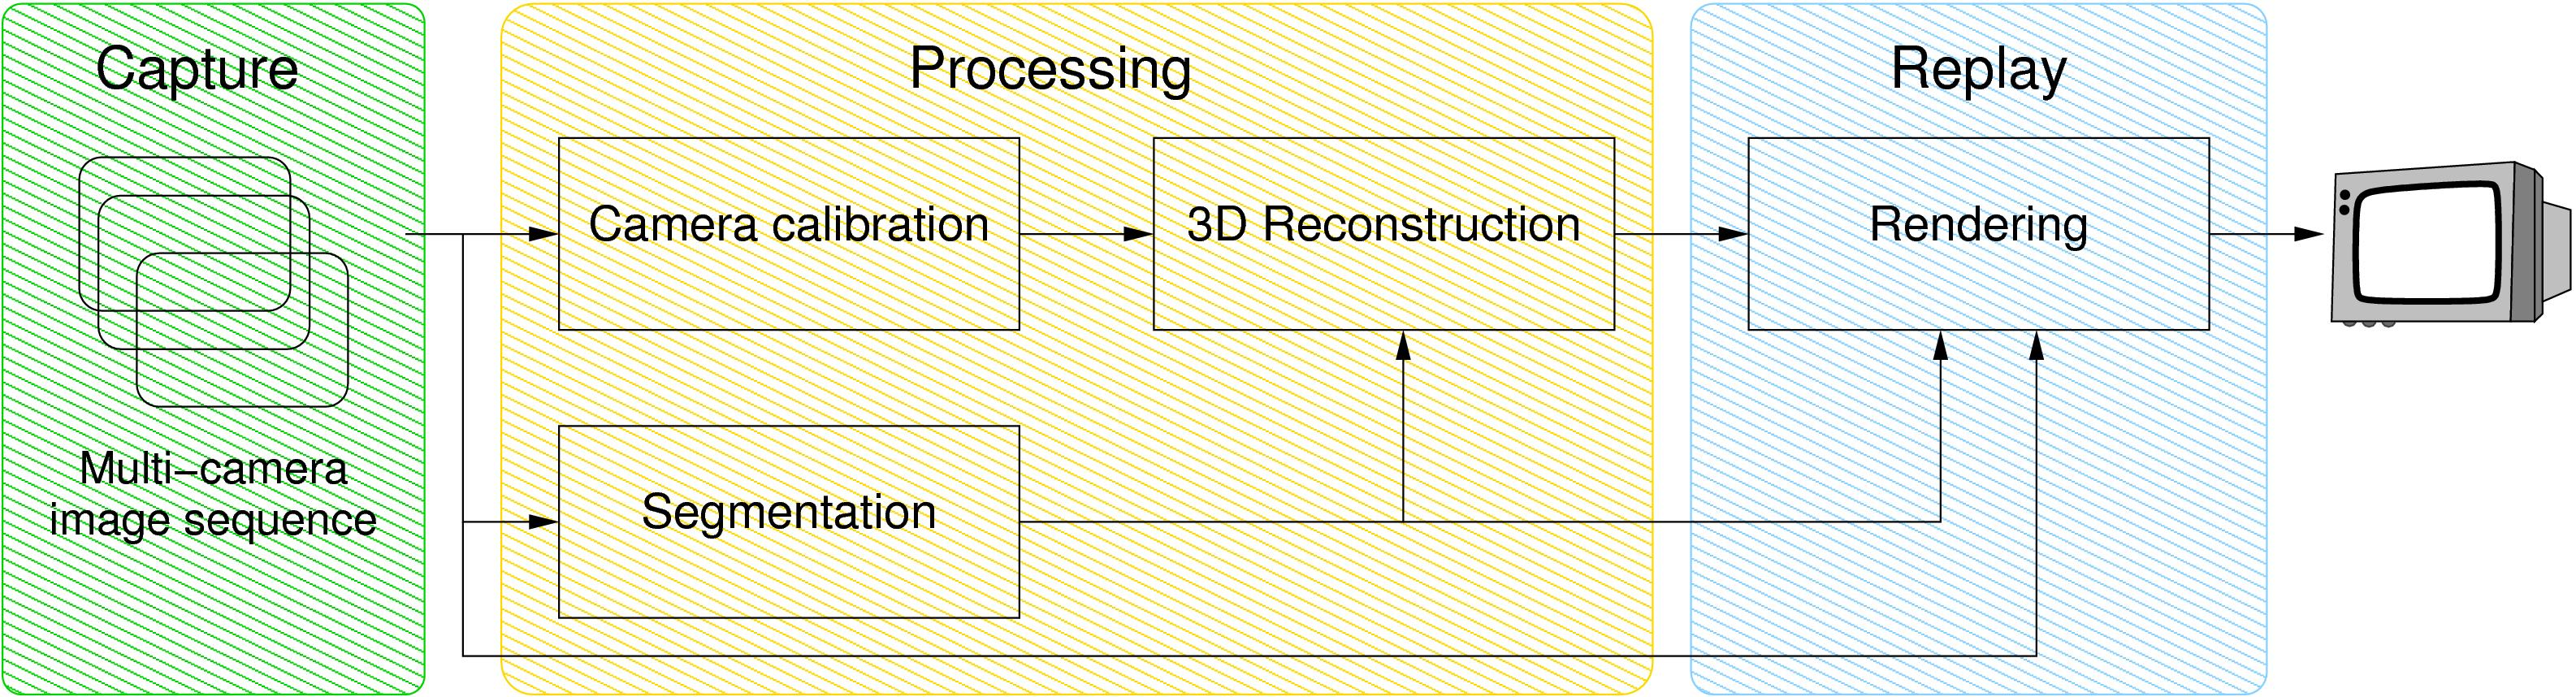
\includegraphics[scale=0.078]{iview_overview2.png}}
\caption{Overview of the \textit{iview} free-viewpoint video system \cite{02_iview}.}
\label{fig:iview_overview}
\end{figure}


The \textit{iview} system is composed of three main modules as shown in Figure \ref{fig:iview_overview}: 
capture, processing and replay module.

Capture is performed using time synchronised acquisition from both auxiliary and
match cameras.
The minimal number of cameras is about four, but for good quality results a higher number is required.
Camera synchronisation is achieved using standard genlock process.

The processing module computes a 3D model of the scene.
This is done using segmentation of objects from the background and 3D reconstruction \cite{2.1_iview}.

To allow the use of footage from match cameras and to avoid the need for prior calibration, 
automatic calibration of all cameras is performed using a line-based approach against the pitch lines of the captured footage, 
achieving a root-mean-square error of 1-2 pixels for moving cameras. 
The calibration is very fast and robust, capable of real-time operation for use during live match footage. 
Calibration estimates the extrinsic and intrinsic parameters of each camera including lens distortion.

The segmentation is needed to separate the foreground, i.e., the players, from the background.
Matting of players from the green pitch is performed using chroma-keying matting. 
% This allows the approximate segmentation of the foreground players for subsequent processing to produce free-viewpoint video. 
The authors developed and tested a k-nearest neighbour approach for chroma-keying and evaluated two other known techniques,
\textit{Fast green subtraction} in RGB colour space and keying in HSV colour space.
The k-nearest neighbour classifier is controlled by a GUI where the user has to click on position in the image that corresponds
to the background. 
The process is repeated until the resulting segmentation is satisfying.
A deeper explanation is present in the paper \cite{2.1_iview} where the authors present and evaluate also 
\textit{Fast green subtraction} and keying in HSV.

The accumulation of errors from calibration and matting can cause large errors in
the reconstruction of the scene, such as loss of limbs. 
Therefore, robust algorithms have been developed for scene reconstruction.
One possible technique is called visual-hull (VH) and represents the maximum volume occupied by an object
given a set of silhouettes from multiple views \cite{2.2_iview_08}.
The visual-hull is a single global representation integrating silhouette information from all
views. A polygonal mesh surface is typically extracted and texture mapped by resampling
the captured multiple view video for rendering \cite{2.2_iview}.
Due to accumulating errors in camera calibration and segmentation, visual-hull accuracy is reduced.
A refinement of the view-dependent visual hull (VDVH) \cite{2.1_iview_12},
using stereo correspondence to interpolate between captured
views, can be used to overcome these issues, achieving the best alignment between adjacent views and 
hence improving visual quality.
More information about \textit{iview} 3D reconstruction can be found in \cite{02_iview,2.1_iview,2.2_iview}.

Finally, the replay module renders the novel view of the scene using the computed 3D model together with the
original camera images.
Cameras closer to the virtual viewpoint are chosen to generate the novel viewpoint.
% TODO: può essere descritto maggiormente the replay module 


The method proposed achieves an image quality comparable to that of the input images and it is robust to the
wide-baseline moving camera views at different resolutions.
Calibration and segmentation are very important in order to obtain an overall good quality of the system.
Degradation in image quality will also occur if there are insufficient views for reconstruction.
% TODO: si può aggiungere contenuto

% Aperture correction is also applied to each video sequence to correct for the camera edge enhancement
% used in standard broadcast footage \cite{iview}.

% Likewise matting in relatively uncontrolled outdoor conditions with changing illu-
% mination achieves a segmentation within 1-2 pixels of the true foreground with the
% addition of background clutter for the crowd, hoardings and on-pitch advertising.





% The replay module renders the captured scene in realtime
% using the computed 3D model and the original camera images
% deploying view-dependent texture mapping [8].
% The entire system can potentially operate in real-time. At
% the current stage the processing is done offline. That means
% the images are stored and the processing is run at a later stage.
% The replay module is designed to work at interactive rates.
% \section{Image-based rendering - extended plane sweeping}

% \begin{figure*}[htbp]
% \centerline{\includegraphics[scale=0.18]{plane_sweeping.png}}
% \caption{}
% \label{fig:plane_sweeping}
% \end{figure*}

\begin{figure*}[htbp]
\centerline{\includegraphics[scale=0.18]{plane_sweeping2.png}}
\caption{Overview of the extended plane sweeping method. Both the non real-time and real-time phase are shown \cite{05_plane_sweeping}.}
\label{fig:plane_sweeping2}
\end{figure*}

In this section, we present the work of Goorts et al. \cite{05_plane_sweeping}, i.e., an image-based approach to generate 
virtual camera view interpolating real camera images.
Instead of performing 3D reconstruction, image-based methods directly generate the image of the novel viewpoint.
When multiple cameras are present, plane sweeping can be used \cite{05_plane_sweeping_yang} for both small and wide 
baseline setups.
Plane sweeping has already been used for novel viewpoint in soccer scenes. Goorts et al. \cite{05_plane_sweeping_2013} 
present a method with two plane sweeps and a depth filtering step suitable for smaller baseline 
setups of about 1 meter. 
This method presents some problems like disappearing players
when they overlap in the image.

The method presented here is fully automatic and employs GPU
parallel processing to achieve fast processing speed.
The system setup consists of 7 static cameras placed in a
wide baseline setup, i.e., 10 meters between each camera.
All cameras are synchronized on shutter level using a global clock.
% All images are transferred to a storage server,
% where all the captured data is stored. A render com-
% puter can access all required images to generate a
% novel viewpoint.
The generation of novel viewpoint consists of two steps as shown in Figure \ref{fig:plane_sweeping2}:
a first off-line preprocessing phase and a real-time interpolation phase. 

The preprocessing phase is responsible for camera calibration and background determination.
Cameras are calibrated in order to acquire their position, orientation and extrinsic and intrinsic parameters.
The calibration method of Svoboda et al. \cite{05_plane_sweeping_Svoboda} has been employed for this purpose:
SIFT features are extracted from a number of frames and the pairwise matching between them is calculated 
using the k-d tree algorithm; these matches are tracked across different image pairs obtaining point 
correspondences between multiple images \cite{05_plane_sweeping}.
The background of every image stream is determined using a per-pixel median approach applied to about 30 images
per stream (2 seconds apart each other).


The real-time phase generates images for a chosen virtual camera position and a chosen time in the video sequence.
First, camera images are debayered and segmented. These images are then used to process foreground and background independently.
The foreground rendering uses a plane-sweep approach followed by depth filtering and a depth-selective plane sweep 
as explained in \cite{05_plane_sweeping}.
The foreground and background are then merged together according to the segmentation information.

Debayering consists of converting the raw images to its RGB representation.
Segmentation is based on backgrounds obtained during off-line preprocessing and is performed on a per-pixel basis using
the differences between the color values and three thresholds.
This allows fast segmentation in high quality.


Applying this method, the authors obtained high quality results using wide baseline setup and typical artifacts of normal plane sweeping, 
such as ghost players, are removed.
Some other artifacts can still be present, such as ghost lines, caused by the simplified assumption of the geometry of the pitch.
% , where the
% reprojection consistency for different depths is maxi-
% mized, thus generating a novel image and depth map
% simultaneously. However, normal plane sweeping
% does not yield high quality results for soccer scenes
% using a wide baseline setup. Serious artifacts, such as
% ghost players, can be perceived. Therefore, we em-
% ploy a depth selection method where the acceptable
% depths of groups of pixels is determined and used in a
% second, depth-selective plane sweep.
% To demonstrate our method, we obtained images
% from a real soccer match in real conditions. Our
% method outperforms other free viewpoint video sys-
% tems, as demonstrated by the results and the accompa-
% nying video. Typical artifacts, such as ghost players,
% are effectively removed.
% \section{Billboard-based visualization}
In this section, we present the work of Ohta et al. \cite{03_billboard}.
The authors use billboard representation to make a 3D model of each player.
This method is simpler than full 3D reconstruction and requires less computation.
A player billboard is a small rectangle standing perpendicular to the ground
and a 2D texture is shown on it.
The difference between 3D reconstruction and billboard representation is shown in Figure \ref{fig:billboard_comparison}:
as we can see, the visual difference is clear at a close viewpoint but becomes very small at a distant one.
For this reason, becomes particularly important to place player billboards at a right place and direction.

\begin{figure}[htbp]
\centerline{\includegraphics[scale=0.22]{billboard_comparison.png}}
\caption{Appearance similarity between 3D reconstruction and billboard in close and distant view \cite{03_billboard}.}
\label{fig:billboard_comparison}
\end{figure}


The system proceeds as follows: first it extracts texture segments from camera videos, then selects appropriate textures according
to the virtual viewpoint and finally layouts the player billboards in virtual space.

Texture extraction phase consists in obtaining the location of each player and extracting texture segments from every image 
video by projecting player location onto the image plane.
Background region is removed in the texture by video capturing PC.
Please note that camera calibration is done before this phase.

Texture selection phase selects a set of texture to be sent to each viewer based on his viewpoint. 
Given a viewpoint, the system finds the camera that minimizes the angle between the line from the viewpoint to the player 
location and the line from the camera to the player location. Then, a texture segment obtained by that camera is selected 
and placed so that the texture faces the viewpoint \cite{03_billboard}.
% TODO: completare


One problem may happen when players are overlapped each other at a certain camera and billboard texture might include both
of them.
To eliminate extra player region, authors used stereo based method \cite{03_billboard_04} as explained in \cite{03_billboard}. 
% TODO: can be explained more



% \section{Conclusion}
We have briefly presented three free-viewpoint systems for soccer games: the \textit{iview} system, an image-based method using 
plane sweeping and a billboard-based method.

The \textit{iview} system is a robust method using a multi-camera setup that performs 3D reconstruction exploiting a refinement 
of the view-dependent visual hull method.
% This method requires % TODO: finire

The image-based method presented interpolates real camera images using a plane sweeping approach.
High quality images using wide baseline setup are obtained and typical artifacts are removed.

The billboard-based method is simpler than full 3D reconstruction and requires less computation.
However, this method produces lower quality images and some visual artifacts can be present.





\bibliographystyle{IEEEtran}
\bibliography{biblio.bib}



\end{document}